%!TEX root = ../Thesis.tex
%% Basierend auf TeXnicCenter-Vorlage von Mark Müller
%%                      Willi Nüßer
%%                      Waldemar Penner     
%%                      Ulrich Reus
%%                      Frank Plass
%%                      Oliver Tribeß 
%%                      Daniel Hintze     
%%%%%%%%%%%%%%%%%%%%%%%%%%%%%%%%%%%%%%%%%%%%%%%%%%%%%%%%%%%%%%%%%%%%%%%

% Wählen Sie die Optionen aus, indem Sie % vor der Option entfernen  
% Dokumentation des KOMA-Script-Packets: scrguide

%%%%%%%%%%%%%%%%%%%%%%%%%%%%%%%%%%%%%%%%%%%%%%%%%%%%%%%%%%%%%%%%%%%%%%%
%% Optionen zum Layout des Artikels                                  %%
%%%%%%%%%%%%%%%%%%%%%%%%%%%%%%%%%%%%%%%%%%%%%%%%%%%%%%%%%%%%%%%%%%%%%%%
\documentclass[%
paper=A4,         % alle weiteren Papierformat einstellbar
fontsize=12pt,    % Schriftgröße (12pt, 11pt (Standard))
BCOR12mm,         % Bindekorrektur, bspw. 1 cm
DIV14,            % breiter Satzspiegel
parskip=half*,    % Absatzformatierung s. scrguide 3.1
headsepline,      % Trennline zum Seitenkopf  
%footsepline,     % Trennline zum Seitenfuß
%normalheadings,  % Überschriften etwas kleiner (smallheadings)
listof=totoc,     % Tabellen & Abbildungsverzeichnis ins Inhaltsverzeichnis      
%bibtotoc,        % Literaturverzeichnis im Inhalt 
%draft            % Überlangen Zeilen in Ausgabe gekennzeichnet
footinclude=false,% Fußzeile in die Satzspiegelberechnung einbeziehen 
headinclude=true, % Kopfzeile in die Satzspiegelberechnung einbeziehen 
final             % draft beschleunigt die Kompilierung
]
{scrartcl}

%\setuptoc{toc}{totoc} % Inhaltsverzeichnis ins Inhaltsverzeichnis

% Neue Deutsche Rechtschreibung und Deutsche Standardtexte
\usepackage[ngerman]{babel} 

% Umlaute können verwendet werden
\usepackage[utf8]{inputenc}   

% Echte Umlaute
\usepackage[T1]{fontenc} 

% Latin Modern Font, Type1-Schriftart für nicht-englische Texte
\usepackage{lmodern} 

% 1/2-zeiliger Zeilenabstand
\usepackage[onehalfspacing]{setspace}

% Für die Defenition eigener Kopf- und Fußzeilen
\usepackage{fancyhdr} 

% Für die Verwendung von Grafiken
\usepackage[pdftex]{graphicx}

% Bessere Tabellen
\usepackage{tabularx}

% Für die Befehle \toprule, \midrule und \bottomrule, z.B. in Tabellen 
\usepackage{booktabs}

% Erlaubt die Benutzung von Farben
\usepackage{color}

% Links im PDF
\usepackage{hyperref}

% Verbessertes URL-Handling mit \url{http://...}
\usepackage{url}

% Listen ohne Abstände \begin{compactlist}...\end{compactlist}
\usepackage{paralist} 

% Ausgabe der aktuellen Uhrzeit für die Draft-Versionen
\usepackage{datetime}

% Deutsche Anführungszeichen
\usepackage[babel,german=quotes]{csquotes}

% Verbessert das Referenzieren von Kapiteln, Abbildungen etc.
\usepackage[german,capitalise]{cleveref}

% Konfiguration der Abbildungs- und Tabellenbezeichnungen
\usepackage[format=hang, font={footnotesize, sf}, labelfont=bf, justification=raggedright,singlelinecheck=false]{caption}

% Verbessert die Lesbarkeit durch Mikrotypografie
\usepackage[activate={true,nocompatibility},final,tracking=true,kerning=true,spacing=true,factor=1100,stretch=10,shrink=10]{microtype}  

% Zitate und Quellenverzeichnis
\usepackage[
    style=authoryear,         % Zitierstil
    firstinits=false,         % false = Vornamen werden ausgeschrieben
    natbib=true,
    urldate=long,             % "besucht am" - Datum
    %url=false,
    date=long,                
    dashed=false, 
    maxcitenames=3,           % max. Anzahl Autorennamen in Zitaten
    maxbibnames=99,           % max. Anzahl Autorennamen im Quellenverzeichnis
    %backend=bibtex           % Ggf. für ältere Distributionen bibtex verwenden
]{biblatex}

% Bibliograpthy
\bibliography{library/library}

% Keine Einrückung bei einem neuen Absatz
\parindent 0pt 

% Ebenentiefe der Nummerierung
\setcounter{secnumdepth}{3}

% Gliederungstiefe im Inhaltsverzeichnis 
\setcounter{tocdepth}{3} 

% Tabellen- und Abbildungsverzeichnis mit Bezeichnung:
\usepackage[titles]{tocloft}
\renewcommand*\cftfigpresnum{Abbildung~}
\renewcommand*\cfttabpresnum{Tabelle~}
\renewcommand{\cftfigaftersnum}{:}
\renewcommand{\cfttabaftersnum}{:}
\settowidth{\cftfignumwidth}{\cftfigpresnum 99~\cftfigaftersnum}
\settowidth{\cfttabnumwidth}{\cfttabpresnum 99~\cftfigaftersnum}

% Style für Kopf- und Fußzeilenfelder
\pagestyle{fancy}
\fancyhf{}
\fancyhead[R]{\leftmark}
\fancyfoot[R]{\thepage} 
\renewcommand{\sectionmark}[1]{\markboth{#1}{#1}} 
\fancypagestyle{plain}{}

% Macro für Quellenangaben unter Abbildungen und Tabellen
\newcommand{\source}[1]{{\vspace{-1mm}\\\footnotesize\textsf{\textbf{Quelle:}} \textsf{#1}\par}}

% Sourcecode-Listings
\usepackage{listings}

% Bestimmte Warnungen unterdrücken
% siehe http://tex.stackexchange.com/questions/51867/koma-warning-about-toc
\usepackage{scrhack} 

% Anpassungen der Formatierung an Eclipse-Aussehen 
% http://jevopi.blogspot.de/2010/03/nicely-formatted-listings-in-latex-with.html
%\definecolor{sh_comment}{rgb}{0.12, 0.38, 0.18 } %adjusted, in Eclipse: {0.25, 0.42, 0.30 } = #3F6A4D
%\definecolor{sh_keyword}{rgb}{0.37, 0.08, 0.25}  % #5F1441
%\definecolor{sh_string}{rgb}{0.06, 0.10, 0.98} % #101AF9
% Für Druckausgabe sollte alles schwarz sein
\definecolor{sh_comment}{rgb}{0.0, 0.0, 0.0 }
\definecolor{sh_keyword}{rgb}{0.0, 0.0, 0.0 }
\definecolor{sh_string}{rgb}{0.0, 0.0, 0.0 }

\lstset{ %
  language=Java,
  basicstyle=\small\ttfamily,
  fontadjust, 
  xrightmargin=1mm,
  xleftmargin=5mm,
  tabsize=2,
  columns=flexible,
  showstringspaces=false,
  rulesepcolor=\color{black},
  showspaces=false,showtabs=false,tabsize=2,
  stringstyle=\color{sh_string},
  keywordstyle=\color{sh_keyword}\bfseries,
  commentstyle=\color{sh_comment}\itshape,
  captionpos=t,
  lineskip=-0.3em
}

\renewcommand{\lstlistingname}{Listing}
\renewcommand\lstlistlistingname{Listingverzeichnis}

\makeatletter
\def\l@lstlisting#1#2{\@dottedtocline{1}{0em}{1em}{\lstlistingname\space{#1}}{#2}}
\makeatother

% Anhangsverzeichnis
\usepackage[nohints]{minitoc} %Anhangsverzeichnis

\makeatletter
\newcounter{fktnr}\setcounter{fktnr}{0}
\newcounter{subfktnr}[fktnr]\setcounter{subfktnr}{0}

\renewcommand\thesubfktnr{\arabic{fktnr}.\thefktnr}
\newcounter{anhangcounter}
\newcommand{\blatt}{\stepcounter{anhangcounter}}

\newcommand{\anhang}[1]{\setcounter{anhangcounter}{0}\refstepcounter{fktnr}
\addcontentsline{fk}{subsection}{Anhang~\thefktnr: \hspace*{1em}#1}
\subsection*{{Anhang~\thefktnr \hspace*{1em} #1 \hspace*{-1em}}}
}

\newcommand{\subanhang}[1]{\setcounter{anhangcounter}{0}\refstepcounter{subfktnr}
\addcontentsline{fk}{subsubsection}{Anhang~\thesubfktnr: \hspace*{1em}#1}
\subsubsection*{{Anhang~\thesubfktnr \hspace*{1em} #1 \hspace*{-1em}}}
}

\newcommand{\anhangsverzeichnis}{\mtcaddsection{\subsection*{Anhangsverzeichnis \@mkboth{FKT}{FKT}}}\@starttoc{fk}\newpage}

% Abkürzungsverzeichnis
\usepackage[acronym,         % create list of acronyms
            nonumberlist,
            toc, 
            section,
            nomain,          % don't need main glossary for this example
            hyperfirst=false,% don't hyperlink first use
            sanitize=none    % switch off sanitization as description
            ]{glossaries}
            \newglossarystyle{mylist}{%
\glossarystyle{long}% base this style on the list style
\renewcommand*{\glossaryentryfield}[5]{%
    \glsentryitem{##1}\textbf{##2} & ##3 \\}%
}

\newacronym{AES}{AES}{Advanced Encryption Standard}
\newacronym{AI}{AI}{Artificial Intelligence}
\newacronym{AOA}{AOA}{Angle of Arrival}
\newacronym{API}{API}{Application Programming Interface}
\newacronym{ATM}{ATM}{Automated Teller Machine}
\makeglossaries\makeglossaries

%%%%%%%%%%%%%%%%%%%%%%%%%%%%%%%%%%%%%%%%%%%%%%%%%%%%%%%%%%%%%%%%%%%%%%%
%% Parameter - Hier auf die eigene Arbeit anpassen
%%%%%%%%%%%%%%%%%%%%%%%%%%%%%%%%%%%%%%%%%%%%%%%%%%%%%%%%%%%%%%%%%%%%%%%

\newcommand{\dokumententyp}{Studienarbeit}
\newcommand{\abgabedatum}{\today} 
\newcommand{\ort}{Mettmann} 
\newcommand{\koorperationsunternehmen}{Unternehmen GmbH}
\newcommand{\dokumententitel}{Entwicklung eines Softwareprojektes}
\newcommand{\dokumentensubtitel}{Spiele Lizenzschlüssel Preisvergleich}
\newcommand{\dokumentenautorA}{Niklas Hardes}
\newcommand{\dokumentenautorB}{Nicolas Groß}
\newcommand{\dokumentenautorC}{Robert Hesselmann}
\newcommand{\dokumentenautoradressA}{A}
\newcommand{\dokumentenautoradressAB}{A}
\newcommand{\dokumentenautoradressB}{Winkelstraße 66}
\newcommand{\dokumentenautoradressBB}{45966 Gladbeck}
\newcommand{\dokumentenautoradressC}{Kronprinzenstraße 83}
\newcommand{\dokumentenautoradressCB}{40217 Düsseldorf}
\newcommand{\dokumentenpruefer}{Dr. Thomas Ströder}
\newcommand{\studiengang}{Angewandte Informatik}
\newcommand{\spezialisierungsbereich}{A}
\newcommand{\matnummerA}{000000}
\newcommand{\matnummerB}{101669}
\newcommand{\matnummerC}{101672}

%%%%%%%%%%%%%%%%%%%%%%%%%%%%%%%%%%%%%%%%%%%%%%%%%%%%%%%%%%%%%%%%%%%%%%%

\hypersetup{
  colorlinks=false,
  pdfborder={0 0 0},
  pdftitle=\dokumententitel~\dokumentensubtitel,
  pdfauthor=\dokumentenautorA\,\dokumentenautorB\,\dokumentenautorC
} 

\begin{document}

% Römische Seitennummerierung
\pagenumbering{Roman}
 
%%%%%%%%%%%%%%%%%%%%%%%%%%%%%%%%%%%%%%%%%%%%%%%%%%%%%%%%%%%%%%%%%%%%%%%
%% Titelseite
%%%%%%%%%%%%%%%%%%%%%%%%%%%%%%%%%%%%%%%%%%%%%%%%%%%%%%%%%%%%%%%%%%%%%%%

%!TEX root = ../Thesis.tex

\begin{titlepage}

\begin{center}


\includegraphics[scale=1.20]{img/fhdw}\\

\ort\\

\vspace{.7cm}

\large{\bfseries\dokumententyp}

~\vspace{.1cm}\\

\LARGE{\dokumententitel}

~\vspace{.1cm}\\

\large{

Prüfer:\vspace{1mm}\\

\dokumentenpruefer

\vspace{1cm}

Verfasser:\\\vspace{1mm}

\dokumentenautor\\
\dokumentenautoradress


\begin{center}
    \begin{tabular}{rcl} 
       Matrikelnummer &:& \matnummer\\
       \vspace{1cm}\\
       Studiengang &:& \studiengang \\ 
       Spezialisierungsbereich &:& \spezialisierungsbereich \\ 
    \end{tabular}
\end{center} 


\vspace{1.5cm}

Abgabetermin:\\

\abgabedatum

}

\end{center}


\end{titlepage}



%%%%%%%%%%%%%%%%%%%%%%%%%%%%%%%%%%%%%%%%%%%%%%%%%%%%%%%%%%%%%%%%%%%%%%%
%% Draft-Einstellungen
%%
%% Für die finale Version auskommentieren!
%%%%%%%%%%%%%%%%%%%%%%%%%%%%%%%%%%%%%%%%%%%%%%%%%%%%%%%%%%%%%%%%%%%%%%%
%\fancyhead[L]{\color{red} Stand: \today~-~\currenttime}

%%%%%%%%%%%%%%%%%%%%%%%%%%%%%%%%%%%%%%%%%%%%%%%%%%%%%%%%%%%%%%%%%%%%%%%
%% Verzeichnisse
%%%%%%%%%%%%%%%%%%%%%%%%%%%%%%%%%%%%%%%%%%%%%%%%%%%%%%%%%%%%%%%%%%%%%%%


% Sperrvermerk
%!TEX root = ../Thesis.tex
\section*{Sperrvermerk}
\addcontentsline{toc}{section}{Sperrvermerk}
\fancyhead[R]{Sperrvermerk}

Diese Thesis enthält vertrauliche Informationen über die Firma \koorperationsunternehmen. Die Weitergabe des Inhalts dieser Arbeit (auch in Auszügen) ist untersagt. Es dürfen keinerlei Kopien oder Abschriften - auch nicht in digitaler Form - angefertigt werden. Auch darf diese Arbeit nicht veröffentlicht werden und ist 
ausschließlich dem Erst- und Zweitprüfer, Mitarbeitern der Verwaltung und Mitgliedern des Prüfungsausschusses sowie auf Nachfrage einer Evaluierungskommission zugänglich zu machen. Personen, die Einsicht in diese Arbeit erhalten, verpflichten sich, über die Inhalte dieser Thesis und all ihren Anhängen keine Informationen, die die \koorperationsunternehmen{} betreffen, gegenüber Dritten preiszugeben. Ausnahmen bedürfen der schriftlichen Genehmigung der \koorperationsunternehmen.
\newpage
\fancyhead[R]{\leftmark}

% Inhaltsverzeichnis
\tableofcontents\newpage

% Glossar
\renewcommand{\glossarypreamble}{\label{glossary}}
\printglossary[style=long, title=Glossar, toctitle=Glossar] \newpage

% Abkürzungsverzeichnis
\renewcommand{\glossarypreamble}{\label{acronyms}}
\printglossary[type=acronym, style=long, title=Abkürzungsverzeichnis, toctitle=Abkürzungsverzeichnis] \newpage

\setcounter{table}{0} % printglossary erzeugt eine Tabelle, die die Nummerierung der "echten" Tabellen durcheinander bringt.

%%%%%%%%%%%%%%%%%%%%%%%%%%%%%%%%%%%%%%%%%%%%%%%%%%%%%%%%%%%%%%%%%%%%%%%
% Verzeichnisse
%%%%%%%%%%%%%%%%%%%%%%%%%%%%%%%%%%%%%%%%%%%%%%%%%%%%%%%%%%%%%%%%%%%%%%%

% Abbildungsverzeichnis
\fancyhead[R]{\listfigurename}
\listoffigures\newpage

% Tabellenverzeichnis
\fancyhead[R]{\listtablename}
\listoftables\newpage

% Quelltextverzeichnis
\renewcommand{\lstlistlistingname}{Quelltextverzeichnis}
\fancyhead[R]{\lstlistlistingname}
\lstlistoflistings\newpage

% Kapitelüberschriften für den Arbeitstext
\fancyhead[R]{\leftmark}

%%%%%%%%%%%%%%%%%%%%%%%%%%%%%%%%%%%%%%%%%%%%%%%%%%%%%%%%%%%%%%%%%%%%%%%
%% Inhalt
%%%%%%%%%%%%%%%%%%%%%%%%%%%%%%%%%%%%%%%%%%%%%%%%%%%%%%%%%%%%%%%%%%%%%%%

% Arabische Seitennummerierung
\pagenumbering{arabic} 

%!TEX root = ../Thesis.tex
\section{Einleitung}


%!TEX root = ../Thesis.tex
\section{UserStories \& Use Cases}

\subsection{User Story}

\subsubsection{Niklas Hardes}

Ich als Gamer möchte wissen, welche Spiele am beliebtesten sind, am meisten gespielt werden und infolgedessen für mich am interessantesten sein können.

\subsection{Robert Hesselmann}

Ein erfolgreicher Streamer auf der Livestreaming Plattform Twitch sucht nach neuen Spielen, die er in seinen Livestreams Spielen kann. Um seinen Gewinn zu maximieren sucht er nach einem Spiel zu einem günstigen Preis.

\subsection{Use Case}


\subsection{Robert Hesselmann}

\begin{figure}[hbt]
    \centering
    \begin{minipage}[t]{1\textwidth} % Breite, z.B. 1\textwidth		
        \caption{Use Case Streamer} % Überschrift
        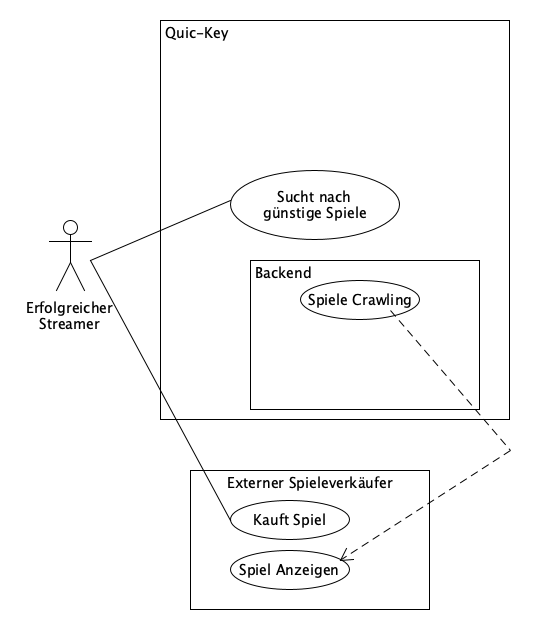
\includegraphics[width=1\textwidth]{img/use_case_streamer.png}\\ % Pfad
        \source{Eigene Darstellung} % Quelle
    \end{minipage}
\end{figure}

% !TeX root = ../Thesis.tex

\section{Technologieentscheidungen}

%!TeX root = ../Thesis.tex

\section{Entwicklungsprinzipien}

\subsection*{Nicolas Groß}

Modularisierung ist die Unterteilung eines Systems in kleinere Module. Die Modularisierung bietet Eigenschaften, welche bei der Entwicklung und Wartung von Software, Vorteile einbringen.  Zu diesen Vorteilen zählen Verständlichkeit, Kombinierbarkeit, Lokalität und die parallele Entwicklung. Die Verständlichkeit einer Software wird durch die Modularisierung verbessert, da einzelne Bestandteile weitgehend unabhängig von anderen Bestandteilen gekapselt und verständlich sind. Die einzelnen Module einer Software können auf unterschiedliche Arten miteinander kombiniert werden, um neue Systeme zusammenzufügen. Dies bietet den Vorteil das Module idealerweise unabhängig vom restlichen System funktionieren und wiederverwendet werden können. Durch die Lokalität zeichnet sich aus, dass Änderungen an einzelnen Modulen keine größeren Änderungen im Gesamtsystem zufolge haben. Ein entscheidender Vorteil für die Entwicklung im Team ist die Möglichkeit zur parallelen Entwicklung. Hierbei können einzelne Teammitglieder an unterschiedlichen Modulen arbeiten, ohne mit den Entwicklungen der anderen Mitglieder zu kollidieren. Das System wird dann zu einem späteren Zeitpunkt zusammengesetzt.\footcite[.vgl]{Schmidauer2002}

Durch Angular ist eine hohe Modularisierung bereits von Beginn des Projekts gegeben, da die Angular-CLI Komponenten und Services in einzelnen Dateien erzeugen. Auch die Projektstruktur wird von der Angular-CLI angepasst, um Komponenten und Services anzulegen. Die einzelnen Komponenten können durch die Verwendung von Variablen wiederverwendbar gestaltet werden, um diese beliebig zu kombinieren. Die Änderungen an einer Komponente haben hierbei in der Regel keinen Einfluss auf andere Komponenten oder Services, wodurch Änderungen meist leicht umgesetzt werden können und dennoch Projektweit geltend sind.

\subsection*{Single-Responsibility Prinzip (Niklas Hardes)}

Bei dem Single-Responsibility Prinzip lautet die Kern-Definition \glqq Ein Modul sollte einem, und nur einem, Akteur gegenüber verantwortlich sein.\grqq{}. Es ist ein wichtiger Bestandteil der SOLID-Prinzipien der objektorientierten Programmierung. Es bedeutet, dass jede Klasse, Methode oder Funktion in einem Programm nur eine einzige Verantwortung hat.

Dem entgegen steht ein sogenanntes God-Object. Es hat viele Verantwortungen und wirkt sich auf unterschiedliche Bereiche aus.
Das macht es schwierig, dieses zu verstehen, zu testen und zu warten. Des Weiteren kann es aufwendig sein, alle Auswirkungen im Blick zu behalten, die eine Änderung an diesem mit sich bringen würde. Insofern ist es sehr zu empfehlen, die Verantwortlichkeiten gering zu halten bzw. im Idealfall nur eine einzige zu haben.

Ebenfalls gibt es Auswirkungen auf Abhängigkeiten zwischen Klassen. Wenn eine Klasse mehrere Verantwortungen hat, kann es viele Abhängigkeiten zu anderen Klassen geben, die die Wartbarkeit des Codes beeinträchtigen können. Eine Klasse mit einer einzigen Verantwortung hat jedoch in der Regel weniger Abhängigkeiten, was die Wartbarkeit des Codes verbessert.

Zusammenfassend, unter Einhaltung des SRP sollte jede Klasse, Methode oder Funktion nur eine einzige Verantwortung haben. Dies erleichtert es, Änderungen an einer Klasse vorzunehmen, ohne Auswirkungen auf andere Teile des Systems zu haben, und die Abhängigkeiten zwischen Klassen zu minimieren.

Das beste Beispiel liefert hierzu unsere Implementation des ThreadedWebSocket im Namespace QuicKey.Business.Web. Es besitzt eine geringe Anzahl an Abhängigkeiten, welche ebenfalls über Interfaces ausgetauscht werden können und somit gut testbar sind. Seine einzige Verantwortlichkeit liegt dabei, die Kommunikation über ein WebSocket zu ordnen, zu steuern und anderen Klassen zur Verfügung zu stellen.

% !TeX root = ../Thesis.tex

\section{Visualisierte Sichten auf das Gesamtsystem}

\subsection*{Gesamtsystem Use-Case Diagramm (Niklas Hardes)}

Im Folgenden ein Use-Case Diagramm als Visualisierung zum Gesamtsystem:

\begin{figure}[hbt!]
%\centering
    \begin{minipage}[t]{.7\textwidth} % Breite, z.B. 1\textwidth		
        \caption{Use-Case Diagramm Gesamt System} % Überschrift
        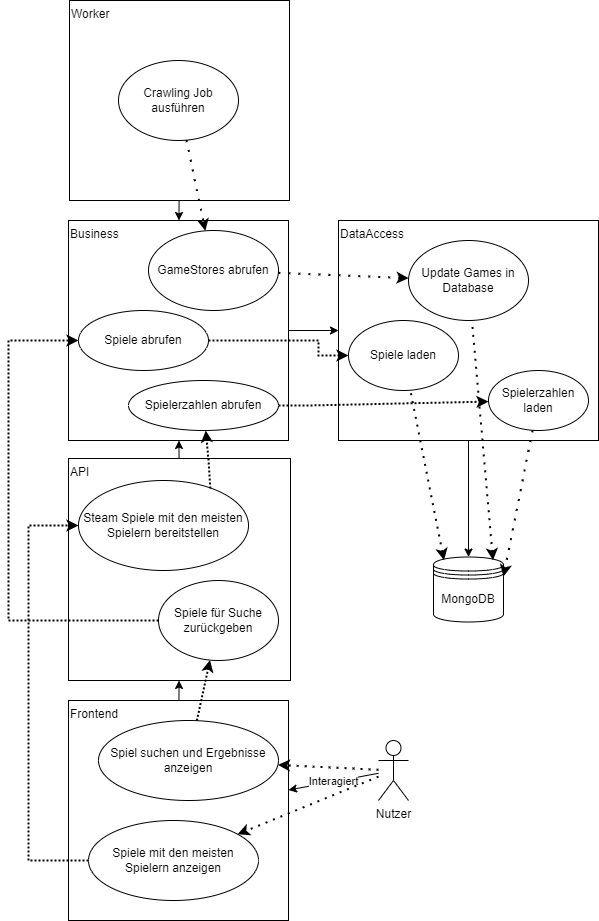
\includegraphics[width=1\textwidth]{img/use_case_gesamt_system.png}\\ % Pfad
        \source{Eigene Darstellung} % Quelle
    \end{minipage}
\end{figure}

% !TeX root = ../Thesis.tex

\section{Entwurfsmuster}

\subsection*{Nicolas Groß}

Bei Anwendungen wie in unserem Fall, einer Single-Page-Application (SPA), werden alle Teile auf einmal geladen, um dem Nutzer ein möglichst flüssiges Erlebnis zu bieten. Dadurch werden häufig auch unbenutzte Module der Anwendung geladen. Bei kleineren Projekten stellt dies keine Probleme da, allerdings kann es bei größeren Projekten zu langen Ladezeiten führen. Um dem entgegenzuwirken, bietet sich Lazy Loading. Beim Lazy Loading werden Inhalte einer Anwendung erst geladen, sobald sie benötigt werden. Dadurch werden Wartezeiten beim Start der Anwendung verkürzt.
In Angular haben Module die Möglichkeit via Lazy Loading geladen zu werden. Durch den entsprechenden Code im Routing-Module wird das Lazy Loading auf die Module angewendet.

\begin{figure}[bht]
\begin{lstlisting}[caption=Codeausschnitt des Tabs Routingmodule,language=json]
{
  path: 'home',
  loadChildren: () => import('../tab1/tab1.module')
                        .then(m => Tab1PageModule),
  data: {
    title: 'Home', 
    icon: 'home'
  }
}
\end{lstlisting}
%\footnoterule{}
%\footnotesize{Casts have been omitted for the sake of readability}
\end{figure}

Wie in diesem Codeausschnitt zu sehen, wird das Modul erst beim Aufruf der Route importiert und geladen. Somit wurde Lazy Loading in Angular-Routing implementiert.\footcites[.vgl]{LazyLoading2021}

Neben dem Routing bedienen wir uns noch zwei weiter Male den Lazy Loading. Der von Ionic bereitgestellte HTML-Tag „<ion-img>“, welche zum Anzeigen Bildern verwendet wird, lädt Bilder standardmäßig über Lazy Loading. Den deutlichsten unterschied der Ladezeiten weist allerdings die InfinityScroll der „Search“-Seite auf. Bei einer Suche werden die Einträge paketweise der Liste hinzugefügt. Weiter Einträge werden erst der Liste erst hinzugeladen, sobald der Nutzer bis kurz vorm unteren Ende der Liste scrollte.\footcites[.vgl]{Ionic2013b}

\subsection*{Fluent-Interfaces (Niklas Hardes)}

In der Softwareentwicklung sind Fluent-Interfaces ein Entwurfsmuster, das darauf abzielt, den Code lesbarer und verständlicher zu machen, indem es die Verkettung von Methoden ermöglicht. Sie sind besonders nützlich für die Erstellung von komplexen und hierarchischen Objekten.

In unserem Projekt haben wir für das Backend die Sprache C\# gewählt. In dieser Sprache werden diese Ketten dadurch ermöglicht, dass Methoden das eigene Objekt zurückgeben, wodurch weitere Methoden direkt hintereinander aufgerufen werden können.

Wir haben dieses Muster unteranderem benutzt, um HTTP Anfragen auf einfache Art konstruieren zu können.
Dazu haben wir die Klasse CustomHttpRequest angelegt, welche dann Methoden wie die SetHeader besitzt.

\begin{figure}[bht]
\begin{lstlisting}[caption=Codeausschnitt von CustomHttpRequest (1),language=json]
public CustomHttpRequest SetHeader(string key, string value)
{
    this._headers ??= new Dictionary<string, string>();
    this._headers[key] = value;
    return this;
}
\end{lstlisting}
%\footnoterule{}
%\footnotesize{Casts have been omitted for the sake of readability}
\end{figure}

Diese Methode konfiguriert bzw. modifiziert die Header des Requests und gibt sich selber zurück, wodurch weitere Methoden aufgerufen werden können. Ein vollständiger Aufruf könnte dann wie folgt aussehen.

\begin{figure}[bht]
\begin{lstlisting}[caption=Codeausschnitt von CustomHttpRequest (2),language=json]
_requester.BuildRequest(HttpMethod.Get, "https://api.steampowered.com/ISteamApps/GetAppList/v2/")
            .SetHeader("User-Agent", "QuicKey Worker")
            .SetCookie("testCookie", "testValue")
            .Request()
\end{lstlisting}
%\footnoterule{}
%\footnotesize{Casts have been omitted for the sake of readability}
\end{figure}

In dem Konstruktor bzw. der Factory Methode werden die benötigten Attribute wie die Methode und die Uri, welche zwingend benötigt werden direkt übergeben. Diese Methode gibt dann ein Objekt der Klasse CustomHttpRequest zurück. Bei diesem Objekt wird dann mithilfe eines Fluent-Interfaces ein exemplarischer Header und Cookie gesetzt. Am Ende wird dann die Request Methode aufgerufen, wodurch die Kette abgeschlossen, die Anfrage gestellt und das Ergebnis der Anfrage zurückgegeben wird. Dies ist dann kein CustomHttpRequest mehr, sondern eine HttpResponseMessage.


% !TeX root = ../Thesis.tex

\section{Architekturstile}

\subsection*{Model-View-ViewModel Architektur (Nicolas Groß)}

Die Model-View-ViewModel Architektur (MVVM) ist ein Konzept der Softwarearchitektur und ist eine Variation der Model-View-Controller Architektur (MVC). Diese Architektur unterscheidet zwischen Model, der View und dem ViewModel.

Das Model enthält die Struktur der Daten und dient zur Erhaltung und Validierung der dem Nutzer anzuzeigenden und von ihm manipulierten Daten. Ein weiterer Nutzen des Models ist die Bereitstellung weiterzuleitender Daten zum Speichern in einer Datenbank. Das Model enthält keine Prozesslogik, sondern ausschließlich die Datenstruktur der Daten. Das Model ist nach einem objektorientierten Prinzip angelegt und kann zum Beispiel wie folgt aufgebaut sein:

\begin{figure}[bht]
\begin{lstlisting}[caption=Codeausschnitt des GameModel Interfaces,language=json]
export interface GameModel{
  refLink: string;
  timestamp: string;
  name: string;
  price: number;
  priceUnit: string;
  imageLink: string;
  storePlatform: string;
}
\end{lstlisting}
%\footnoterule{}
%\footnotesize{Casts have been omitted for the sake of readability}
\end{figure}

Hier ist das im Projekt verwendete GameModel definiert, welches zum Laden und Anzeigen der Spiele aus der Datenbank verwendet wird.

Als View bezeichnet man die Benutzeroberfläche, mit welcher der Nutzer interagiert. Diese bestehen im Fall von Angular aus Templates. Diese Templates werden durch HTML und CSS strukturiert und gestaltet. Zudem enthalten sie Variablen, welche sich an die Daten des ViewModel binden, um diese anzuzeigen.

Das ViewModel enthält die Logik der UI-Komponenten. Das ViewModel greift auf Methoden und Dienst des Models zu und stellt zudem auch benötigte Informationen, Eigenschaften und Methoden zur Verwendung in der View bereit.

Angular folgt dem Prinzip der MVVM-Architektur. Komponenten in Angular bestehen immer aus zwei Teilen, dem Template und der Logik. Komponenten zeichnen sich durch ein „@Component“ im ViewModel aus. Das sieht zum Beispiel wie folgt aus:

\begin{figure}[bht]
\begin{lstlisting}[caption=Codeausschnitt der SearchPageComponent,language=json]
@Component({
  selector: 'app-search-page',
  templateUrl: './search-page.component.html',
  styleUrls: ['./search-page.component.scss'],
})
export class SearchPageComponent implements AfterViewInit {...}
\end{lstlisting}
%\footnoterule{}
%\footnotesize{Casts have been omitted for the sake of readability}
\end{figure}

Hier werden ein Tag der Komponente („selector“) zum Aufruf in Templates, der Pfad zur Template-Datei („templateUrl“) und der Pfad zu einer zusätzlichen Style-Datei („styleUrls“) angegeben. Durch diese Angaben werden View und ViewModel miteinander verknüpft.


\subsection*{Master-Slave-Architektur / Client-Server-Architektur (Niklas Hardes)}

Bei dem Abfragen von Spiele-Händlern ergab sich das Problem, dass diese Limitierungen eingebaut haben, wonach die Anfragen pro IP-Adresse eingeschränkt sich. Dafür hatten wir 2 Lösungen. Die Erste wäre die Geschwindigkeit stark zu reduzieren, was allerdings dennoch schnell zu einem Ban führen würde, da das Abfragen dennoch überwacht wird und ein Sequenzielles Abfragen sehr auffällig ist.
Die 2. Option ist es die Anzahl an IP-Adressen zu erhöhen und dann wie sehr viele Nutzer auszusehen.

Diese 2. Option wurde dann gewählt. Dazu baut der Worker eine WebSocket Verbindung mit einem Vermittlungsserver auf. Dieser Server nimmt die Anfragen entgegen, leitet sie an hunderte Slaves weiter, welche diese Anfrage durchführen und dann die Antwort an den Vermittlungsserver zurückgeben.
Dieser gibt die Antworten dann über das WebSocket an den Worker zurück, wo dann diese verarbeitet und in die Datenbank eingepflegt werden.

Einerseits stellt dies eine Client-Serververbindung dar zwischen unserem Worker und dem Vermittlungsserver. Andererseits eine Master-Slave-Architektur, da die Anfragen auf viele kleine Slaves verteilt werden. Im Allgemeinen gibt es in dieser einen Master, der die Kontrolle über eine Gruppe von Slaves hat. Der Master ist dafür verantwortlich, die Anfragen der Slaves zu verwalten und sicherzustellen, dass die Slaves die Anforderungen erfüllen. Dies passiert in unserem Fall noch mit einer Zwischenstelle.


\subsection*{Schichtenarchitektur (Robert Hesselmann)}

Unsere Software haben wir mit Hilfe der Schichtenarchitektur gestaltet. Die Software ist geteilt in die Datenschicht, die Businessschicht und die Zugriffsschicht.

Die Datenschicht repräsentiert mit Hilfe von Entities die Datenbank, die Datenbank bekommt nur Anfragen über die Datenschicht.

Die Businessschicht oder auch Businesslogik genannt, beinhaltet alle Logischen Operationen mit den Daten und der Verarbeitung der Daten.

Die Zugriffsschicht gibt die Daten nach Außen weiter, bspw. mit einer \gls{http}-Schnittstelle.

\include{chapter/Gegenüberstellungen}


% %!TEX root = ../Thesis.tex
\section{Grundlagen}

\subsection{Schrift}
\label{sec:schrift}

\subsubsection{Schriftgrößen}
\label{sec:schriftgroessen}
\tiny Das ist sehr kleine Schrift\\
\small Das ist kleine Schrift\\
\normalsize Das ist normale Schrift\\
\large Das ist große Schrift\\
\Large Das ist größere Schrift\\
\LARGE Das ist noch größere Schrift\\
\huge Das ist riesige Schrift\\
\Huge Das ist noch riesigere Schrift\\
\scriptsize Das ist Script Schrift\\
\footnotesize Das ist Fußnoten Schrift
\normalsize

\subsubsection{Schrift Typen}
\label{sec:Schrift Typen}
\textbf{Das ist ein fetter Text}\\
\textit{Das ist ein kursiver Text}\\
\underline{Das ist ein unterstrichener Text}\\
\textsc{Das ist ein kapitälchen Text}\\
\textsf{Das ist ein serifenloser Text}\\
\texttt{Das ist ein Schreibmaschinen Text}\\
\textnormal{Das ist ein normaler Text}

\subsubsection{Schrift Ausrichtung}
\label{sec:Schrift Ausrichtung}
\begin{quote}
Quote Text (Der gesamte Text innerhalb der Umgebung wird von beiden Seiten eingerückt)
\end{quote}
\begin{center}
Zentrierter Text (Der gesamte Text innerhalb der Umgebung wird zentriert)
\end{center}
\begin{flushleft}
Linksbündiger Text (Der gesamte Text innerhalb der Umgebung wird linksbündig)
\end{flushleft}
\begin{flushright}
Rechtsbündiger Text (Der gesamte Text innerhalb der Umgebung wird rechtsbündig)
\end{flushright}
In einer Fußnote\footnote{können zusätzliche Ergänzungen, Präzisierungen, Textverweise usw. eingeführt werden.}

\subsection{Abbildungen}

In \cref{fig:fhdw} sehen Sie das Logo der FHDW.

\begin{figure}[hbt]
\centering
\begin{minipage}[t]{.7\textwidth} % Breite, z.B. 1\textwidth		
\caption{Das Logo der FHDW} % Überschrift

\includegraphics[width=1\textwidth]{img/fhdw.pdf}\\ % Pfad
\source{Eigene Darstellung} % Quelle
\label{fig:fhdw}
\end{minipage}
\end{figure}

\subsection{Tabellen}

In \cref{tab:pin} auf Seite \pageref{tab:pin} sehen Sie die am häufigsten benutzten PINs.

\begin{table}[hbt]
\centering
\begin{minipage}[t]{.5\textwidth} % Breite, z.B. 1\textwidth		
\caption{Die am häufigsten verwendeten PINs} % Überschrift
\begin{tabularx}{\columnwidth}{rXrr}
\toprule
Rank & PIN & Percentage & Accumulated \\
\midrule
1 & 1234 & 4.34\% & 4.34\%\\
2 & 0000 & 2.57\% & 6.91\%\\
3 & 2580 & 2.32\% & 9.23\%\\
4 & 1111 & 1.60\% & 10.83\%\\
5 & 5555 & 0.87\% & 11.70\%\\
6 & 5683 & 0.70\% & 12.39\%\\
7 & 0852 & 0.60\% & 12.99\%\\
8 & 2222 & 0.56\% & 13.55\%\\
9 & 1212 & 0.49\% & 14.03\%\\
10 & 1998 & 0.43\% & 14.46\%\\
\bottomrule
\end{tabularx}
\source{Eigene Darstellung} % Quelle
\label{tab:pin}
\end{minipage}
\end{table}

\subsection{Zitate}

Ein Zitat im Fließtext ist zu sehen bei \citet{Fuller2011}.

Ein vergleichendes Zitat.\footnote{\cite[vgl.][5\psqq]{Maslennikov2011}}

Ein \enquote{wörtliches Zitat}\footnote{\cite[13\psq]{Meier2010}}

Zitat einer Quelle mit mehreren Autoren.\footnote{\cite[vgl.][32\psqq]{Hocking2011a}}


\subsection{Abkürzungen}
Bei der ersten Verwendung werden Abkürzungen ausgeschrieben: \gls{AES}.
Später wird dann automatisch nur noch die Kurzform benutzt: \gls{AES}


\subsection{Listen}
\label{sec:Listen}
Eine einfache List mit Punkten:

\begin{compactitem}
	\item Punkt 1
	\item Punkt 2
	\item Punkt 3
\end{compactitem}

Eine einfache Liste mit Nummern:
\begin{compactenum}
	\item Punkt 1
	\item Punkt 2 
	\item Punkt 3
\end{compactenum}

Eine einfache Liste mit römischen Nummern:
\begin{compactenum}[I.]
	\item Punkt 1
	\item Punkt 2
	\item Punkt 3
\end{compactenum}

Eine einfache Liste mit Buchstaben:
\begin{compactenum}[(a)]
	\item Punkt 1
	\item Punkt 2 
	\item Punkt 3
\end{compactenum}

\subsection{Quelltext}

Listing~\ref{list:android} auf Seite~\pageref{list:android} zeigt einigen Quelltext.

\begin{figure}[bht]
\begin{lstlisting}[caption=Scanning for Wi-Fi Access Points on Android, label=list:android]
registerReceiver(new RSSIBroadcastReceiver(), 
    new IntentFilter(WifiManager.SCAN_RESULTS_AVAILABLE_ACTION));

WifiManager wifi = getSystemService(Context.WIFI_SERVICE);
wifi.startScan();

/* not thread safe */
public class RSSIBroadcastReceiver extends BroadcastReceiver {

    public void onReceive(Context context, Intent intent) {
        WifiManager wifi = getSystemService(Context.WIFI_SERVICE);
        List<ScanResult> scanResults = wifiManager.getScanResults();

        for (ScanResult scanResult : results) {
            RSSI rssi = new RSSI();
            rssi.bssi = scanResult.BSSID;
            rssi.signalLevel = scanResult.level;
        }
    }
}
\end{lstlisting}
%\footnoterule{}
%\footnotesize{Casts have been omitted for the sake of readability}
\end{figure}

%!TEX root = ../Thesis.tex
\section{Zusammenfassung}

Dieses Dokument ist eine Hilfe, um die Formalien für eine Bachelor-Thesis an der
FHDW bei der Verwendung von {\LaTeX} zu erfüllen und dabei möglichst viele Automatismen von {\LaTeX} zu nutzen. Eine Absprache mit dem betreuenden Professor ist dennoch ratsam.

	
%%%%%%%%%%%%%%%%%%%%%%%%%%%%%%%%%%%%%%%%%%%%%%%%%%%%%%%%%%%%%%%%%%%%%%%

%!TEX root = ../Thesis.tex
\section*{Anhang}
\addcontentsline{toc}{section}{Anhang}
\fancyhead[R]{Anhang}

\anhangsverzeichnis

\anhang{Gesprächsnotizen}

\subanhang{Gespräch mit Werner Müller}

Gespräch mit Werner Müller am 01.01.2013 zum Thema XXX:
\begin{compactitem}
   \item Über das gute Wetter gesprochen
   \item Die Regenwahrscheinlichkeit liegt immer bei ca. 3\%
   \item Das Unternehmen ist total super
   \item Hier könnte eine wichtige Gesprächsnotiz stehen
\end{compactitem}


%!TEX root = ../Thesis.tex
\section*{Quellenverzeichnis}
\addcontentsline{toc}{section}{Quellenverzeichnis}
\fancyhead[R]{Quellenverzeichnis}

\defbibheading{mono}{\subsection*{Monographien}}
\defbibheading{mag}{\subsection*{Aufsätze in Sammelbänden und Zeitschriften}}
\defbibheading{art}{\subsection*{Zeitungsartikel}}
\defbibheading{web}{\subsection*{Internetquellen}}
\defbibheading{leg}{\subsection*{Rechtsprechung}}
\defbibheading{comp}{\subsection*{Unternehmensunterlagen/Gesprächsnotizen}}

\setlength\bibitemsep{1.5\itemsep}
\setlength{\bibhang}{2em}

\renewcommand{\baselinestretch}{1.50}\normalsize

\begingroup
\sloppy

\printbibliography[heading=mono,keyword=mono]
\printbibliography[heading=mag,keyword=mag]
\printbibliography[heading=web,keyword=web]

% Bei Bedarf einkommentieren: (erzeugt sonst Warnungen)
% \printbibliography[heading=art,keyword=art]
% \printbibliography[heading=leg,keyword=leg]
% \printbibliography[heading=comp,keyword=comp]

\endgroup


%%%%%%%%%%%%%%%%%%%%%%%%%%%%%%%%%%%%%%%%%%%%%%%%%%%%%%%%%%%%%%%%%%%%%%%

%!TEX root = ../Thesis.tex

\section*{Ehrenwörtliche Erklärung}
\addcontentsline{toc}{section}{Ehrenwörtliche Erklärung}
\fancyhead[R]{Ehrenwörtliche Erklärung}

Hiermit erkläre ich, dass ich die vorliegende \dokumententyp{} selbständig angefertigt habe. Es wurden nur die in der Arbeit ausdrücklich benannten Quellen und Hilfsmittel benutzt. Wörtlich oder sinngemäß übernommenes Gedankengut habe ich als solches kenntlich gemacht. Diese Arbeit hat in gleicher oder ähnlicher Form noch keiner Prüfungsbehörde vorgelegen.
\vspace{20mm}

\ort, \abgabedatum
\vspace{10mm}

\underline{\hspace{8cm}}\\\dokumentenautor
 
%%%%%%%%%%%%%%%%%%%%%%%%%%%%%%%%%%%%%%%%%%%%%%%%%%%%%%%%%%%%%%%%%%%%%%%

\end{document}